\documentclass[11pt,a4paper]{article}
\usepackage[margin=1in]{geometry}
\usepackage{microtype}
\usepackage{setspace}
\usepackage{booktabs}
\usepackage{tabularx}
\usepackage{array}
\usepackage{longtable}
\usepackage{multirow}
\usepackage{enumitem}
\usepackage{graphicx}
\usepackage{amsmath}
\usepackage{amssymb}
\usepackage{xcolor}
\usepackage{hyperref}
\usepackage{cleveref}
\usepackage{tikz}
\usetikzlibrary{arrows.meta,positioning,shapes.geometric,fit,calc}
\usepackage{float}
\usepackage{caption}
\usepackage{subcaption}
\usepackage{fancyhdr}
\usepackage{titlesec}
\usepackage[numbers,sort&compress]{natbib}

\hypersetup{colorlinks=true,linkcolor=black,citecolor=blue,urlcolor=blue}
\setstretch{1.12}
\setlength{\parskip}{0.45em}
\setlength{\parindent}{0pt}
\setlist[itemize]{leftmargin=1.6em,itemsep=0.2em,topsep=0.25em}
\setlist[enumerate]{leftmargin=1.8em,itemsep=0.25em,topsep=0.25em}
\setlength{\headheight}{14pt}
\pagestyle{fancy}
\fancyhf{}
\lhead{Undergraduate Thesis Proposal}
\rhead{Game-State Fusion for Football BAA}
\cfoot{\thepage}
\titleformat{\section}{\large\bfseries}{\thesection.}{0.6em}{}
\titleformat{\subsection}{\normalsize\bfseries}{\thesubsection}{0.6em}{}

\definecolor{softblue}{RGB}{235,244,252}
\definecolor{softgreen}{RGB}{235,248,239}
\definecolor{softorange}{RGB}{253,242,226}
\definecolor{softgray}{RGB}{245,245,245}
\tikzset{
  box/.style={rectangle, rounded corners=3pt, draw=black!65, align=center, minimum height=9mm, text width=28mm, fill=softblue},
  data/.style={rectangle, rounded corners=3pt, draw=black!65, align=center, minimum height=9mm, text width=26mm, fill=softgreen},
  process/.style={rectangle, rounded corners=3pt, draw=black!65, align=center, minimum height=9mm, text width=30mm, fill=softorange},
  decision/.style={diamond, draw=black!65, align=center, aspect=2, fill=softgray, inner sep=1pt},
  arrow/.style={-{Latex[length=2mm]}, thick, draw=black!65}
}

\begin{document}

\begin{titlepage}
\centering
\vspace*{1.0cm}
{\Large \textbf{[University Name]}}\\[0.35cm]
{\large Department of Computer Science and Engineering}\\[1.5cm]

{\LARGE \textbf{Undergraduate Thesis Proposal}}\\[0.8cm]
{\huge \textbf{Evaluating Game-State Fusion for Short-Horizon Ball Action Anticipation in Football}}\\[1.2cm]

\begin{tabular}{ll}
\textbf{Student 1:} & [Name / ID] \\
\textbf{Student 2:} & [Name / ID] \\
\textbf{Student 3:} & [Name / ID] \\
\textbf{Supervisor:} & [Supervisor Name] \\
\end{tabular}

\vfill
\textbf{Prepared: 14 August 2026}\\[0.3cm]
\textit{Primary research direction after literature, dataset, novelty, benchmark, and feasibility audit}
\end{titlepage}

\begin{abstract}
Ball Action Anticipation (BAA) asks a model to predict which ball-related football actions will occur and when they will occur in a short unobserved future interval. Existing BAA work is primarily driven by visual representations, while separate football action-detection and spotting research has shown that explicit game-state information such as player position, velocity, team relation, and multi-player interaction can complement visual evidence when the target action is already observable. This proposal investigates whether that structured information remains useful when the action must be predicted before it occurs.

The proposed study derives a reproducible BAA protocol from SoccerTrack v2, a public dataset containing full-pitch panoramic video, dense game-state reconstruction (GSR), and ball-action spotting (BAS) annotations. The research compares visual-only, game-state-only, simple fusion, flat-relational, and relation-aware fusion models under strict match-level evaluation. The implementation is designed for limited compute: multi-gigabyte GSR JSON files are streamed once into compact state tensors, 4K video is sampled once through a frozen visual encoder, and normal training operates only on compact features. Before full-scale paid compute is used, a 10-minute mini-pilot will validate the entire raw-data-to-prediction pipeline and measure actual resource consumption. The central contribution is therefore a controlled empirical answer to whether explicit player-level game state provides complementary predictive value for short-horizon football action anticipation.
\end{abstract}

\tableofcontents
\newpage

\section{Background and Motivation}
Football video understanding has progressed from action spotting and player tracking toward predictive tasks that ask what will happen next. FAANTRA introduced football Ball Action Anticipation on SoccerNet, predicting future ball actions in unobserved frames over short anticipation windows \citep{dalal2025faantra}. SoccerNet 2026 subsequently formalized a challenge in which 30 seconds of observed football context are followed by a 5-second future interval containing the events to be anticipated \citep{cioppa2026soccernet}.

BAA is attractive for tactical analysis, automated broadcasting, decision-support systems, and intelligent indexing because it operates before an event becomes visible. However, future action prediction is inherently uncertain. Visual evidence alone may not explicitly represent the spatial relationships that make an action likely, such as the distance between attackers and defenders, pressure near the ball, supporting runs, or the collective shape of the two teams.

Separate work demonstrates that explicit football game state can help action understanding. Ochin et al. combine player game state and visual features with a graph-based model for spatio-temporal action detection \citep{ochin2025gamestate}. Beyond Pixels extends observed-action reasoning with game-state and longer temporal context \citep{ochin2025beyond}, while FOOTPASS makes multi-agent tactical context central to player-centric spotting \citep{ochin2025footpass}. These works establish that structured state is useful prior art. They also prevent this thesis from claiming that player graphs, game-state fusion, or multimodal football understanding are new by themselves.

The unresolved question targeted here is narrower: \textit{does synchronized explicit player-level game state help when the target action is still in an unobserved future interval?}

\section{Problem Statement}
Given a historical observation window from a football match, the model must predict a variable-size set of ball actions occurring during the following 5 seconds. Each predicted event contains:
\begin{enumerate}
  \item an action class,
  \item a temporal position within the future interval, and
  \item a confidence/actionness score.
\end{enumerate}
The task is not next-action classification. More than one action may occur in a 5-second future interval, so the prediction head must support set prediction.

The benchmark will provide up to 30 seconds of historical context for compatibility with the SoccerNet 2026 BAA framing \citep{cioppa2026soccernet}. The initial model will consume a shorter recent context, beginning at 5 seconds, because the original FAANTRA study indicates that simply increasing visual context is not automatically beneficial and increases compute \citep{dalal2025faantra}. Context length is therefore a modeling variable rather than a fixed novelty claim.

\section{Research Gap and Novelty Boundary}
\subsection{What prior work already establishes}
\begin{enumerate}
  \item Football Ball Action Anticipation exists and can predict action class and time in unseen future frames \citep{dalal2025faantra,cioppa2026soccernet}.
  \item Video plus explicit player game state already exists for observed-action football detection \citep{ochin2025gamestate}.
  \item Longer temporal and game-level structured context already exists for observed-action denoising/detection \citep{ochin2025beyond}.
  \item Multimodal and multi-agent tactical context already exists in football spotting research \citep{ochin2025footpass}.
  \item Geometry-based football prediction exists in other tasks, including set-piece tactical reasoning and multi-agent tactical forecasting \citep{wang2024tacticai,rao2026gentac,xu2026tacticgen}.
  \item Future football event prediction also exists from sparse event sequences \citep{simpson2022seq2event,hong2025scoutgpt}.
\end{enumerate}

\subsection{Defensible gap}
The reviewed BAA literature predicts future actions primarily from visual observations and, in recent challenge work, high-level semantic tactical context. In contrast, explicit positions, velocities, team information, and player-interaction structure have been shown to complement visual evidence for tasks in which the target action is already visible. The literature reviewed for this proposal does not establish whether synchronized explicit player game state provides complementary predictive value for temporally localized ball actions occurring in an unobserved future interval. This thesis tests that question directly.

\subsection{Claims deliberately not made}
The proposal does not claim to be the first to use a GNN for football players, the first video plus game-state football model, the first football future-event model, or a SoccerNet leaderboard state-of-the-art system. Relation-aware modeling is treated as a controlled method comparison rather than the central invention.

\section{Research Questions and Hypotheses}
\textbf{RQ1.} Does explicit player-level game-state information improve temporally localized short-horizon BAA compared with visual-only anticipation?

\textbf{RQ2.} Does relation-aware player-interaction modeling provide additional anticipation value beyond simple/flat fusion when the underlying state information is held constant?

\textbf{H1.} Adding explicit game state will improve the mean BAA metric relative to a visual-only baseline.

\textbf{H2.} A relation-aware representation will outperform a flat-relations control that receives the same relational information without message passing.

\textbf{H3.} The effect of game state will differ by action class. This is an exploratory hypothesis. No class-specific improvement is assumed before experiments.

\section{Objectives}
\begin{enumerate}
  \item Build a reproducible derived BAA protocol on SoccerTrack v2.
  \item Validate BAS, GSR, and video alignment using a pinned dataset revision.
  \item Create a compute-efficient preprocessing pipeline for multi-gigabyte GSR JSON and panoramic 4K video.
  \item Establish visual-only and game-state-only anticipation baselines.
  \item Measure whether simple game-state fusion improves visual anticipation.
  \item Measure whether explicit relational features and relation-aware modeling add value beyond flat state.
  \item Report grouped match-level performance, fold variation, per-class AP, and efficiency measures.
  \item Produce a zero-recurring-cost inference demonstration after the research experiments are stable.
\end{enumerate}

\section{Related Work}
\begin{table}[H]
\centering
\caption{Positioning of the most important related work.}
\small
\begin{tabularx}{\textwidth}{p{2.7cm}p{2.4cm}p{2.7cm}X}
\toprule
\textbf{Work} & \textbf{Task} & \textbf{Main input/context} & \textbf{Relevance and remaining difference} \\
\midrule
FAANTRA \citep{dalal2025faantra} & Future BAA & Visual football video & Defines the anticipation task and query-style prediction, but does not use explicit synchronized per-player game state. \\
SoccerNet 2026 \citep{cioppa2026soccernet} & Future BAA challenge & Mainly visual, plus documented semantic tactical context in one method & Official 30s observation / 5s future framing. Reviewed methods do not document metric GSR/player-graph inputs. \\
Ochin et al. \citep{ochin2025gamestate} & Spatio-temporal action detection & Video + positions + velocities + team information + graph & Strongest architectural prior. The target action is observed rather than unobserved future. \\
Beyond Pixels \citep{ochin2025beyond} & Detection/denoising & Player-centric predictions + clean game state + longer context & Weakens novelty of contextual/relational football action modeling, but remains observed-action reasoning. \\
FOOTPASS \citep{ochin2025footpass} & Player-centric spotting & Multimodal, multi-agent tactical context & Further establishes tactical context for spotting, not future BAA. \\
SoccerTrack v2 \citep{scott2025soccertrack} & Dataset for GSR/BAS/MOT & Panoramic 4K + player pitch state + BAS & Provides the synchronized data substrate for the proposed derived anticipation protocol. \\
TacticAI \citep{wang2024tacticai} & Corner-kick tactical prediction/generation & Structured player geometry & Shows geometry-based predictive football reasoning is not new. \\
GenTac \citep{rao2026gentac} & Multi-agent tactical forecasting & Tracking trajectories & Threatens generic tactical forecasting novelty, but not video + GSR BAA. \\
Seq2Event \citep{simpson2022seq2event} & Next-event prediction & Sparse event sequences & Shows future football-event prediction itself is not new. \\
TacticGen \citep{xu2026tacticgen} & Tactical trajectory generation & Large event + tracking corpus & Multi-agent future generation at much larger scale, but a different prediction target. \\
\bottomrule
\end{tabularx}
\end{table}

\section{Research Logic}
\begin{figure}[H]
\centering
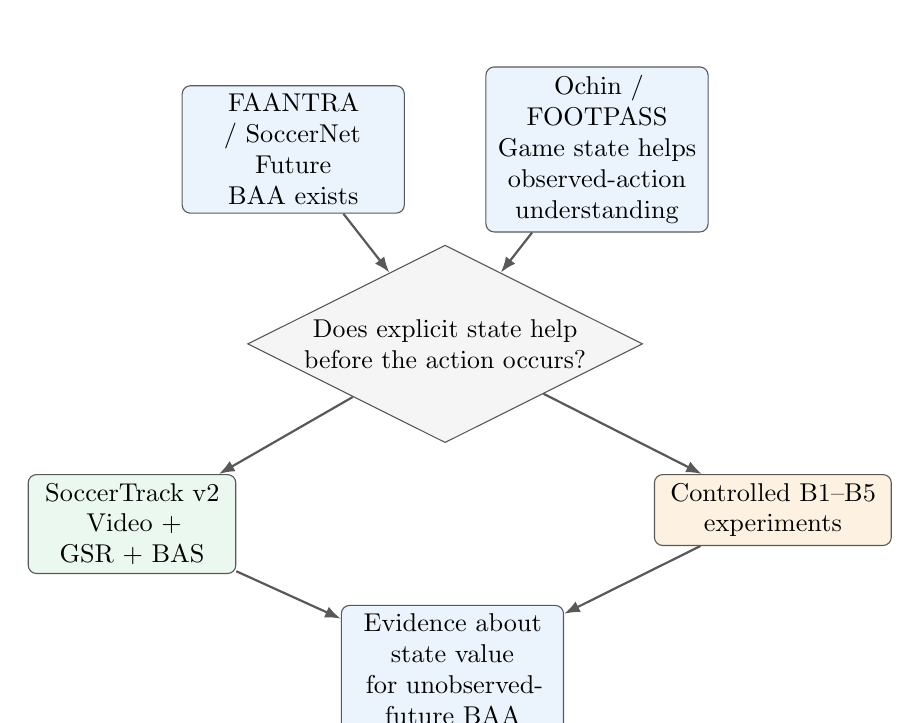
\begin{tikzpicture}[node distance=9mm and 11mm, scale=0.93, transform shape]
\node[box] (f) {FAANTRA / SoccerNet\\Future BAA exists};
\node[box, right=of f] (o) {Ochin / FOOTPASS\\Game state helps observed-action understanding};
\node[decision, below=13mm of $(f)!0.5!(o)$] (q) {Does explicit state help\\before the action occurs?};
\node[data, below left=11mm and 15mm of q] (d) {SoccerTrack v2\\Video + GSR + BAS};
\node[process, below right=11mm and 15mm of q] (e) {Controlled B1--B5\\experiments};
\node[box, below=12mm of $(d)!0.5!(e)$] (c) {Evidence about state value\\for unobserved-future BAA};
\draw[arrow] (f) -- (q);
\draw[arrow] (o) -- (q);
\draw[arrow] (q) -- (d);
\draw[arrow] (q) -- (e);
\draw[arrow] (d) -- (c);
\draw[arrow] (e) -- (c);
\end{tikzpicture}
\caption{Research-gap logic. The thesis tests a bridge between established visual anticipation and established game-state-aware observed-action understanding.}
\end{figure}

\section{Dataset}
\subsection{SoccerTrack v2}
SoccerTrack v2 is a public dataset containing 10 full-length university-level football matches with panoramic 4K video, dense GSR annotations, and BAS annotations for 12 classes \citep{scott2025soccertrack,soccertrackrepo2026}. The GSR includes metric 2D pitch coordinates, player identity/tracking information, roles, and teams. This combination allows the thesis to study future BAA without first training player detection, tracking, re-identification, or camera calibration.

\subsection{Historical local BAS audit}
A previously downloaded Google Drive snapshot was directly audited during topic selection and contained 23,663 BAS events. Pass and Drive dominated the distribution, while Header, Goal, and Free Kick were rare. This count is retained only as provenance and feasibility evidence. It is \textbf{not} treated as the final benchmark count because the Drive-mirror schema differs from the currently documented release structure. Final counts will be regenerated from the pinned experimental revision.

\subsection{Known release-quality safeguards}
The public repository contains evolving documentation and correction notes \citep{soccertrackrepo2026}. The thesis will therefore:
\begin{enumerate}
  \item pin the experimental release/revision,
  \item record file names and hashes when practical,
  \item use project loaders for timestamp semantics,
  \item validate actual shipped schema before writing custom parsers,
  \item quarantine rather than silently delete suspicious annotations, and
  \item resolve or exclude any match with a documented correction that affects the required GSR fields.
\end{enumerate}
Match 132831 is treated as a special audit case because the repository documents a calibration correction issue. Exact benchmark folds are not frozen until this gate passes.

\section{Derived BAA Benchmark Protocol}
\subsection{Task}
Each sample contains up to 30 seconds of available historical context followed by a 5-second unobserved future interval. The target is the set of BAS actions occurring in that future interval.

\subsection{Class policy}
The primary result will use the 10 semantic classes aligned with the established SN-BAA class space by excluding Goal and Free Kick. This is a comparability decision, not a claim that those are the two rarest classes in SoccerTrack v2. A fuller 12-class result will also be reported where statistically meaningful. Rare Header performance will be explicitly visible rather than silently removed after observing model results.

\subsection{Split and leakage policy}
\begin{enumerate}
  \item Split by whole match, never by random windows.
  \item Prefer five-fold grouped evaluation if enough corrected matches remain usable.
  \item No sample crosses half boundaries.
  \item No future video, GSR, or BAS information enters the input.
  \item Normalization and class weights are computed from training matches only.
  \item Player identity is used for trajectory continuity, not as a default semantic learned embedding.
  \item Evaluation windows are generated independently of future-event presence.
\end{enumerate}

\subsection{Metrics}
The evaluation follows BAA-style mean Average Precision at temporal tolerances $\delta=1,2,3,4,5$ seconds and $\delta=\infty$ \citep{dalal2025faantra,cioppa2026soccernet}. For finite $\delta$, a prediction is temporally correct when it falls within $\delta/2$ seconds of the ground-truth time. We will report per-class AP, aggregate mAP, fold mean and dispersion, and avoid comparing absolute SoccerTrack results to the SoccerNet leaderboard because the datasets and domains differ.

\section{Large-Data System Architecture}
The raw dataset is large because dense 25-fps GSR is stored in large JSON files and the video is panoramic 4K. The proposed pipeline therefore converts raw modalities once into compact continuous feature stores.

\begin{figure}[H]
\centering
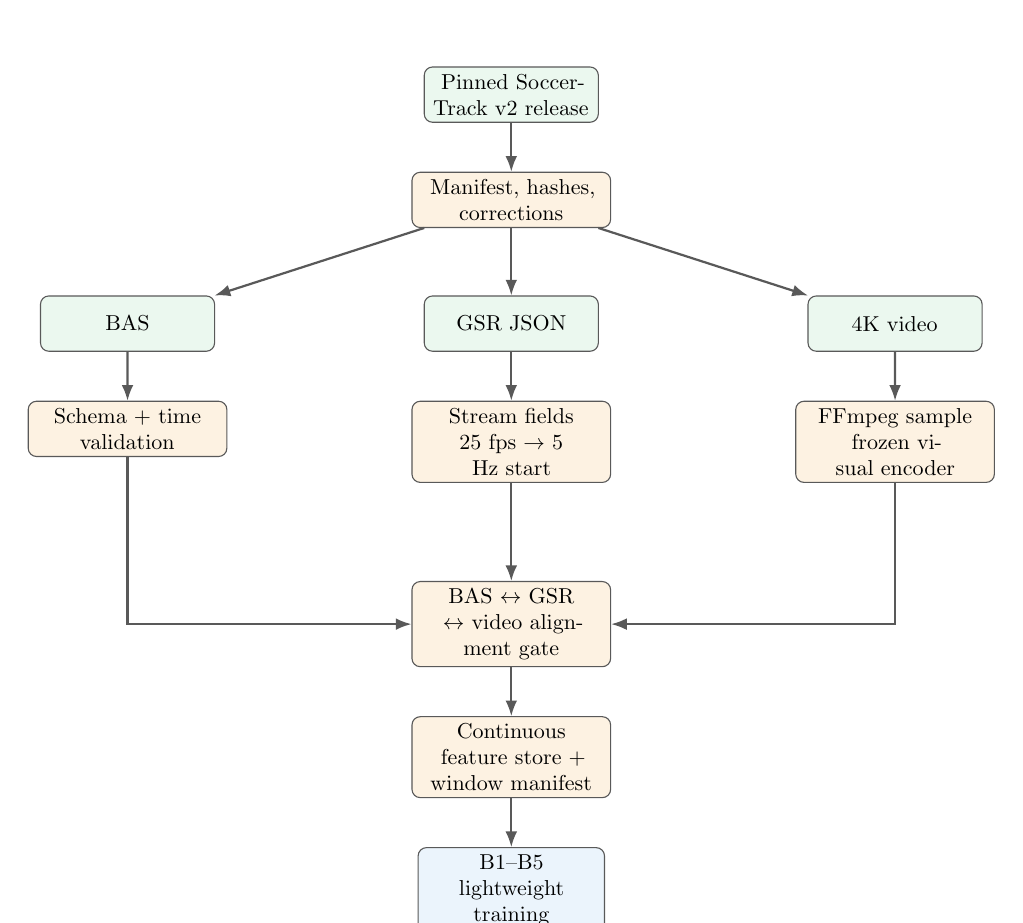
\begin{tikzpicture}[node distance=8mm and 8mm, scale=0.78, transform shape]
\node[data] (src) {Pinned SoccerTrack v2 release};
\node[process, below=of src] (man) {Manifest, hashes, corrections};
\node[data, below left=11mm and 32mm of man] (bas) {BAS};
\node[data, below=11mm of man] (gsr) {GSR JSON};
\node[data, below right=11mm and 32mm of man] (vid) {4K video};
\node[process, below=of bas] (bv) {Schema + time validation};
\node[process, below=of gsr] (gp) {Stream fields\\25 fps $\rightarrow$ 5 Hz start};
\node[process, below=of vid] (vp) {FFmpeg sample\\frozen visual encoder};
\node[process, below=16mm of gp] (align) {BAS $\leftrightarrow$ GSR $\leftrightarrow$ video alignment gate};
\node[process, below=of align] (win) {Continuous feature store + window manifest};
\node[box, below=of win] (train) {B1--B5 lightweight training};
\draw[arrow] (src) -- (man);
\draw[arrow] (man) -- (bas); \draw[arrow] (man) -- (gsr); \draw[arrow] (man) -- (vid);
\draw[arrow] (bas) -- (bv); \draw[arrow] (gsr) -- (gp); \draw[arrow] (vid) -- (vp);
\draw[arrow] (bv) |- (align); \draw[arrow] (gp) -- (align); \draw[arrow] (vp) |- (align);
\draw[arrow] (align) -- (win); \draw[arrow] (win) -- (train);
\end{tikzpicture}
\caption{Raw-dataset-to-model architecture. Large raw files are processed once; model training uses compact aligned artifacts.}
\end{figure}

\subsection{GSR streaming and compression}
The GSR parser will process one half at a time with an incremental parser or official loader. It will keep only task-relevant information: time/frame, player pitch position, role/team relation, tracking identifiers for continuity, and validity masks. Velocity will be derived from historical positions. The first implementation will sample state at 5 Hz. This is an engineering starting point, not a claim of optimal temporal resolution.

A fixed/padded player tensor plus mask will be produced for batching. Continuous per-half arrays will be saved once. Pairwise relations such as relative position, distance, relative velocity, and same-team/opponent indicators can be computed dynamically, preventing a large permanently materialized edge store.

For approximately 900 minutes of football, 5 Hz yields about 270,000 state timestamps. A dense tensor with 22 players and 8 FP16 values per timestamp is only on the order of 100 MiB before metadata and masks, demonstrating why large JSON can become compact model-ready data.

\subsection{Video feature extraction}
Video will be copied/downloaded one match or half at a time, sampled at approximately 6.25 fps as a starting configuration, resized, and passed through a frozen pretrained visual encoder. Embeddings are stored in FP16 with timestamps, then the temporary runtime copy of the raw media can be removed. For roughly 900 minutes, 6.25 fps corresponds to about 337,500 sampled timestamps. A 768-dimensional FP16 representation is roughly 0.5 GiB before metadata, making repeated raw-video decoding unnecessary during training.

\subsection{Window indexing instead of clip duplication}
Overlapping training/evaluation windows will not be saved as separate duplicated tensors. The system stores continuous per-half visual/state arrays and a small table with match, half, context start/end, future start/end, and target-event indexes. The data loader slices these arrays at runtime. This substantially reduces storage and I/O.

\section{Cross-Modal Validation and Double-Checking}
Every BAS event enters the benchmark only after it passes:
\begin{enumerate}
  \item accepted schema under the pinned loader,
  \item known half/segment,
  \item mappable GSR time/frame,
  \item corresponding video time,
  \item no unresolved correction affecting required state.
\end{enumerate}
Failures are recorded with reason codes in an exclusion ledger. The preprocessing stage will generate a dataset manifest, correction log, alignment report, class distribution, per-match counts, usable durations, and final fold manifest.

Approximately 100 randomly sampled aligned events will also receive a manual quality spot-check using the BAS label/time, short video context, and GSR/minimap state. This uses the small manual-review budget as quality assurance rather than as large-scale new annotation.

\section{Proposed Model}
\begin{figure}[H]
\centering
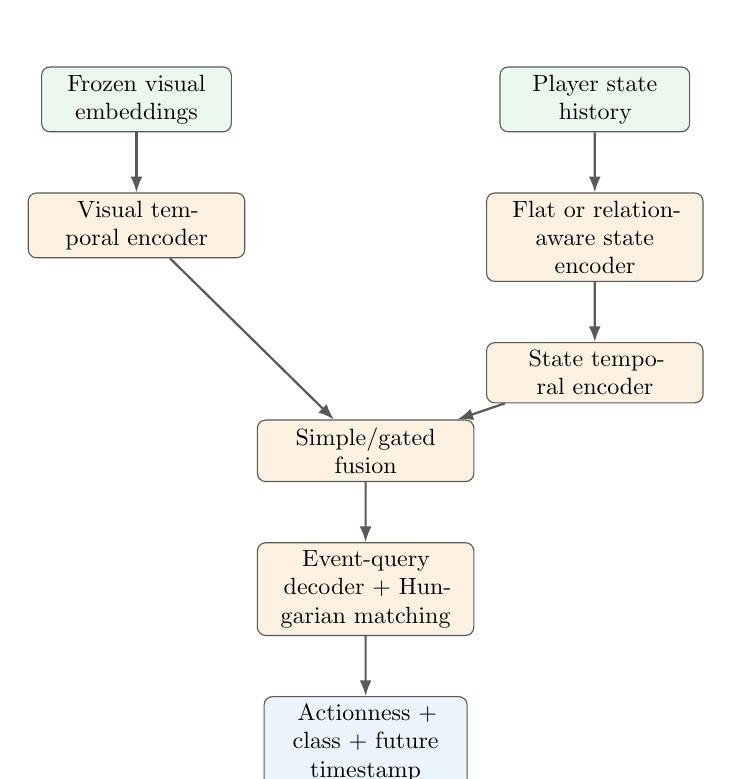
\begin{tikzpicture}[node distance=9mm and 15mm, scale=0.85, transform shape]
\node[data] (v) {Frozen visual embeddings};
\node[process, below=of v] (vt) {Visual temporal encoder};
\node[data, right=40mm of v] (s) {Player state history};
\node[process, below=of s] (rel) {Flat or relation-aware state encoder};
\node[process, below=of rel] (st) {State temporal encoder};
\node[process, below=18mm of $(vt)!0.5!(st)$] (fus) {Simple/gated fusion};
\node[process, below=of fus] (dec) {Event-query decoder + Hungarian matching};
\node[box, below=of dec] (out) {Actionness + class + future timestamp};
\draw[arrow] (v) -- (vt); \draw[arrow] (s) -- (rel); \draw[arrow] (rel) -- (st);
\draw[arrow] (vt) -- (fus); \draw[arrow] (st) -- (fus); \draw[arrow] (fus) -- (dec); \draw[arrow] (dec) -- (out);
\end{tikzpicture}
\caption{Proposed lightweight dual-branch model family. Complexity is intentionally limited so the scientific value comes from controlled comparisons.}
\end{figure}

\subsection{Visual branch}
A frozen visual backbone produces features that are summarized by a small GRU or lightweight temporal encoder. The backbone is not the novelty and will not be repeatedly fine-tuned on 4K frames.

\subsection{Game-state branch}
Player nodes include normalized $x,y$, derived $v_x,v_y$, role, masks, and team relation. Relation-aware variants use local player interactions with features such as $\Delta x$, $\Delta y$, distance, relative velocity, and same-team/opponent indicators. A small message-passing or attention encoder is sufficient. The first design targets two relational layers rather than a deep graph network.

\subsection{Set-prediction head}
A fixed number of event queries predicts actionness, class, and normalized future timestamp. Predictions are matched to variable-size ground-truth event sets using Hungarian matching. Classification can use class weighting; timestamp uses an L1-style regression term; unmatched queries represent no-event slots.

\section{Experiment Matrix}
\begin{table}[H]
\centering
\caption{Core controlled experiment ladder.}
\begin{tabularx}{\textwidth}{p{1.2cm}p{3.2cm}X}
\toprule
\textbf{ID} & \textbf{Model} & \textbf{Scientific purpose} \\
\midrule
B0 & Statistical/no-event floor & Sanity floor for the derived benchmark. \\
B1 & Visual-only BAA & Establish the visual anticipation baseline. \\
B2 & Game-state-only & Test whether explicit state alone contains anticipatory information. \\
B3 & Simple fusion & Test RQ1: whether adding state improves visual-only anticipation. \\
B4 & Flat-relations fusion & Give explicit relational features without graph message passing. \\
B5 & Relation-aware fusion & Test RQ2 by comparing against B4 with equivalent information. \\
\bottomrule
\end{tabularx}
\end{table}

The critical interpretation is B3 versus B1 for the main research question and B5 versus B4 for the relation-model question. If B3 improves while B5 does not beat B4, the thesis can conclude that state is useful without requiring graph reasoning. If B5 fails to beat B1, the result can still show that game-state value observed in detection does not automatically transfer to anticipation.

\subsection{Ablations}
Mandatory comparisons are no-game-state, no-visual-input, and relation-aware versus flat-relations. Velocity and team-relation removals are secondary ablations if time permits. The project explicitly rejects an architecture zoo involving many backbones, graph operators, fusion blocks, frame rates, or context lengths before the core research questions are answered.

\section{Mini Feasibility Prototype}
Before full paid experimentation, a short pilot will prove the entire pipeline on approximately the first 10 minutes of a relatively clean match/half, preferably match 117093 after confirming the pinned release.

\begin{figure}[H]
\centering
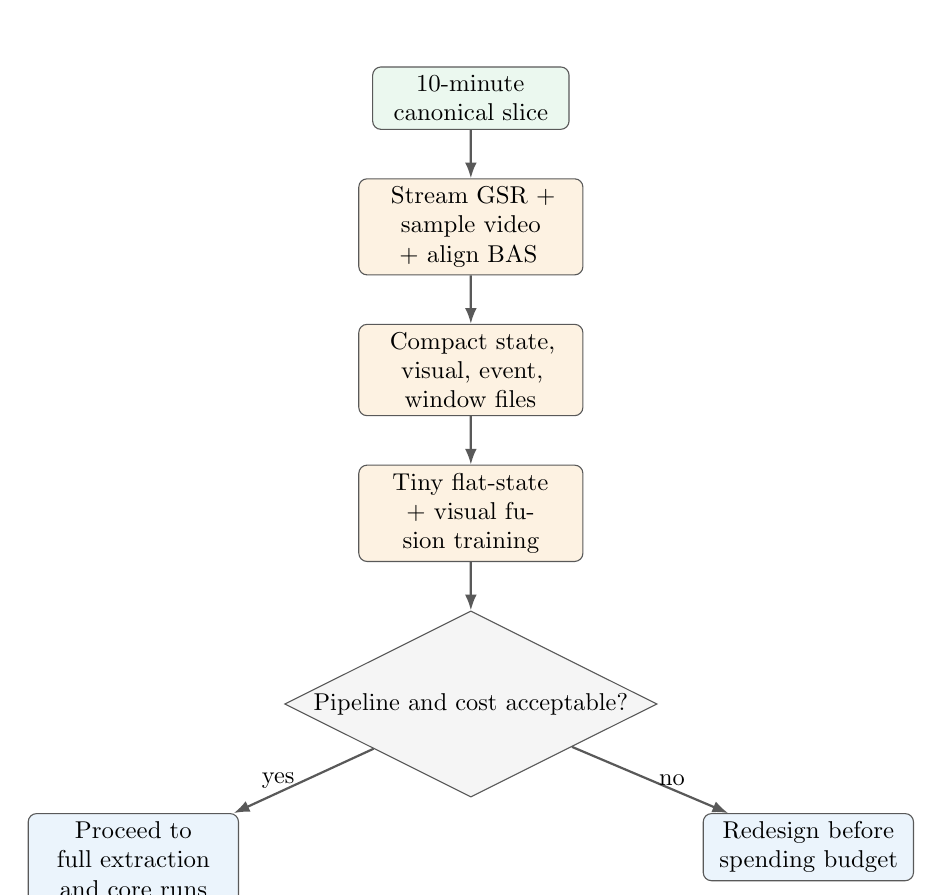
\begin{tikzpicture}[node distance=7mm, scale=0.88, transform shape]
\node[data] (slice) {10-minute canonical slice};
\node[process, below=of slice] (pp) {Stream GSR + sample video + align BAS};
\node[process, below=of pp] (compact) {Compact state, visual, event, window files};
\node[process, below=of compact] (tiny) {Tiny flat-state + visual fusion training};
\node[decision, below=of tiny] (gate) {Pipeline and cost acceptable?};
\node[box, below left=9mm and 20mm of gate] (go) {Proceed to full extraction and core runs};
\node[box, below right=9mm and 20mm of gate] (stop) {Redesign before spending budget};
\draw[arrow] (slice)--(pp); \draw[arrow] (pp)--(compact); \draw[arrow] (compact)--(tiny); \draw[arrow] (tiny)--(gate);
\draw[arrow] (gate)--node[left]{yes}(go); \draw[arrow] (gate)--node[right]{no}(stop);
\end{tikzpicture}
\caption{Feasibility pilot as a go/no-go gate before full paid compute.}
\end{figure}

The pilot must demonstrate successful download/access, streamed GSR parsing, BAS/GSR/video alignment, compact storage, frozen feature extraction, training with finite/decreasing loss, checkpoint save/load, action-class output, timestamp output, and evaluator execution. Accuracy is not a pilot criterion.

The pilot will save a manifest, state tensor, visual features, event/window tables, checkpoint, training log, resource-usage log, and sample predictions. Runtime, peak RAM/VRAM, output size, and accelerator usage are recorded and conservatively extrapolated.

\section{Compute Strategy}
Google Colab provides dynamically allocated GPU/TPU resources and does not guarantee a fixed accelerator type or exact usage limit \citep{googlecolab2026}. Therefore the proposal treats the anticipated 100-unit paid budget as a soft envelope rather than a promise of exact GPU-hours.

\begin{table}[H]
\centering
\caption{Soft accelerator budget. CPU-only work should not consume paid accelerator units where avoidable.}
\begin{tabular}{lr}
\toprule
\textbf{Stage} & \textbf{Soft ceiling} \\
\midrule
Pilot visual extraction & 5 units \\
Remaining full visual extraction & 15 units \\
Pipeline/model debugging & 10 units \\
B1--B5 core experiments & 40 units \\
Essential ablations & 15 units \\
Emergency/re-run reserve & 15 units \\
\midrule
Total envelope & 100 units \\
\bottomrule
\end{tabular}
\end{table}

\subsection{Hard stop rules}
\begin{enumerate}
  \item Measure 10-minute extraction cost before full extraction.
  \item Measure one full match before processing the entire dataset.
  \item Do not launch grouped full evaluation until B1--B5 work on one fold.
  \item Do not spend accelerator units parsing JSON, calculating statistics, or building fold manifests.
  \item If full extraction projects beyond budget, lower frame rate, input resolution, or backbone size before continuing.
  \item Optional ablations begin only after the core research question has an answer.
\end{enumerate}

TPU may be used for a fixed-shape pilot if necessary, but GPU is preferred for the final graph-based pipeline because it reduces framework and dynamic-shape complexity. The system itself is not dependent on TPU availability.

\section{Validation and Statistical Analysis}
Core B1--B5 models should be evaluated across match-grouped folds after the dataset gate is complete. The final report will include:
\begin{enumerate}
  \item mean and dispersion across folds,
  \item per-class AP,
  \item paired fold differences for B3-B1 and B5-B4,
  \item rare-class discussion,
  \item parameter count,
  \item training time per fold,
  \item peak memory,
  \item feature-store size, and
  \item inference latency.
\end{enumerate}
The dataset contains only a small number of independent matches, so statistical claims will remain conservative. The thesis will not present cross-validation as creating more independent matches than actually exist.

\section{Deployment and System Demonstration}
Deployment is a supporting engineering contribution. A short clip or pre-prepared sample is sent to a lightweight FastAPI service, temporarily preprocessed, passed through the anticipation model, and returned as structured predictions such as \texttt{future\_offset}, \texttt{action}, and \texttt{confidence}. Raw uploaded media is deleted after processing. Only compact structured output and model/experiment metadata need to be stored. The target is zero recurring paid infrastructure.

\section{Risk Register and Mitigation}
\begin{longtable}{p{3.2cm}p{5.0cm}p{6.0cm}}
\toprule
\textbf{Risk} & \textbf{Why it matters} & \textbf{Mitigation} \\
\midrule
Dataset schema drift & Different mirrors/revisions may not match documentation. & Pin revision, record hashes, validate shipped schema, use official loaders. \\
Known match correction & A calibration issue can contaminate GSR. & Quarantine affected match until required fields are verified or corrected; otherwise exclude it. \\
Only 10 matches & Single split may be unstable. & Whole-match grouped evaluation and fold dispersion; no window-level random split. \\
Class imbalance & Pass/Drive dominate and rare classes have unstable AP. & Pre-register class policy, class-aware losses, per-class AP, transparent rare-class analysis. \\
Incremental novelty & Video + game-state graphs already exist for detection. & Make future BAA state value the primary research question; B4/B5 control isolates relational modeling. \\
Visual branch adds little & Full-pitch state may already contain much predictive information. & B1/B2/B3 explicitly measure modality contribution. A strong state-only result is scientifically useful. \\
Graph adds little & Relations may help without GNN message passing. & Flat-relations B4 is mandatory before B5. \\
Compute overrun & 4K video and huge JSON can waste budget. & One-time feature extraction, streaming compression, mini pilot, stop rules, reserve units. \\
Domain limitation & University-level full-pitch footage differs from professional broadcast. & Bound conclusions to SoccerTrack v2; no professional-domain generalization claim. \\
Negative result & Fusion may not outperform visual-only. & The design remains valuable because it tests whether detection-time state benefits transfer to anticipation. \\
\bottomrule
\end{longtable}

\section{Reproducibility Plan}
The project will version code in Git and keep raw datasets out of the repository. The release will include configuration files, the dataset manifest, exclusions/corrections, feature-building scripts, benchmark window construction, fold manifests, model configs, training seeds, evaluation scripts, and structured experiment logs. The Obsidian research vault separately preserves decision history and evidence corrections.

The model-ready directory is expected to follow:
\begin{verbatim}
processed/
  manifest/
  events/<match>.parquet
  state/<match>_<half>.npz
  visual/<match>_<half>.npy
  windows/folds.json
  windows/windows.parquet
  audit/alignment_report.json
  audit/class_distribution.json
\end{verbatim}

\section{Expected Contributions}
\begin{enumerate}
  \item \textbf{Primary scientific contribution:} controlled evidence on whether explicit player-level game state improves short-horizon future BAA.
  \item \textbf{Secondary scientific contribution:} evidence on whether relation-aware player interaction modeling adds value beyond flat state and flat relational features.
  \item \textbf{Reproducibility contribution:} a documented procedure for deriving BAA samples from synchronized SoccerTrack v2 video, GSR, and BAS while handling release/version and alignment issues.
  \item \textbf{Engineering contribution:} a compute-efficient raw-data-to-feature-store pipeline and a zero-recurring-cost inference demonstration.
\end{enumerate}

\section{One-Month Execution Plan}
\begin{table}[H]
\centering
\caption{Compressed execution plan.}
\begin{tabularx}{\textwidth}{p{1.5cm}p{4.0cm}X}
\toprule
\textbf{Week} & \textbf{Primary objective} & \textbf{Outputs} \\
\midrule
1 & Data gate + feasibility & Pin release, audit schemas/corrections, 10-minute pilot, cost projection, finalize usable matches/folds. \\
2 & Baselines & Full compact features, B0--B3 on one fold, fix evaluator and losses, then grouped B1--B3 runs. \\
3 & Relation study & B4/B5, essential ablations, per-class analysis, efficiency logging. \\
4 & Writing + demo & Final tables/figures, limitations, FastAPI/demo, thesis proposal/paper expansion, reproducibility release. \\
\bottomrule
\end{tabularx}
\end{table}

\section{Success Criteria}
The thesis is considered scientifically complete if the following are achieved:
\begin{enumerate}
  \item a validated, reproducible SoccerTrack-derived BAA protocol,
  \item at least B1, B2, B3, B4, and B5 evaluated under the same grouped protocol,
  \item clear evidence for or against RQ1,
  \item a controlled result for RQ2,
  \item transparent per-class and fold-level analysis,
  \item documented resource usage and dataset-quality decisions, and
  \item a reproducible code/data-manifest release and small inference demonstration.
\end{enumerate}
A positive accuracy gain is not itself required for thesis validity. The central requirement is an interpretable answer to the research question under a defensible protocol.

\section{Conclusion}
This proposal deliberately narrows novelty to a question that survives the literature and dataset audit. Football BAA already exists; explicit game-state fusion and player-relationship modeling already exist for observed-action tasks; and future football-event prediction exists in other representations. The proposed thesis therefore does not attempt to claim those components as first-time inventions. Instead, it asks whether synchronized explicit player game state provides useful predictive information when the target ball action has not yet occurred. SoccerTrack v2 makes this question experimentally accessible, while streaming structured preprocessing, one-time frozen video feature extraction, controlled B1--B5 baselines, and a pilot-before-paid-compute workflow make the project realistic for an undergraduate team with limited GPU resources.

\newpage
\section*{References}
\addcontentsline{toc}{section}{References}
\begin{thebibliography}{99}

\bibitem[Dalal et al.(2025)]{dalal2025faantra}
M. Dalal, A. Xarles, A. Cioppa, S. Giancola, M. Van Droogenbroeck, B. Ghanem, A. Clapés, S. Escalera, and T. B. Moeslund.
\newblock Action Anticipation from SoccerNet Football Video Broadcasts.
\newblock \emph{CVPR Workshops}, 2025. arXiv:2504.12021.

\bibitem[Cioppa et al.(2026)]{cioppa2026soccernet}
A. Cioppa, S. Giancola, H. Ardö, M. Dalal, J. Held, J. Ochin, J. Rao, K. Sanchez, R. Vandeghen, A. Xarles, et al.
\newblock SoccerNet 2026 Challenges Results.
\newblock \emph{arXiv preprint arXiv:2607.07320}, 2026.

\bibitem[Ochin et al.(2025a)]{ochin2025gamestate}
J. Ochin, G. Devineau, B. Stanciulescu, and S. Manitsaris.
\newblock Game State and Spatio-Temporal Action Detection in Soccer Using Graph Neural Networks and 3D Convolutional Networks.
\newblock \emph{ICPRAM}, pages 636--646, 2025. DOI: 10.5220/0013161100003905.

\bibitem[Ochin et al.(2025b)]{ochin2025beyond}
J. Ochin, R. Chekroun, B. Stanciulescu, and S. Manitsaris.
\newblock Beyond Pixels: Leveraging the Language of Soccer to Improve Spatio-Temporal Action Detection in Broadcast Videos.
\newblock \emph{arXiv preprint arXiv:2505.09455}, 2025.

\bibitem[Ochin et al.(2025c)]{ochin2025footpass}
J. Ochin, R. Chekroun, B. Stanciulescu, and S. Manitsaris.
\newblock FOOTPASS: A Multi-Modal Multi-Agent Tactical Context Dataset for Play-by-Play Action Spotting in Soccer Broadcast Videos.
\newblock \emph{arXiv preprint arXiv:2511.16183}, 2025.

\bibitem[Scott et al.(2025)]{scott2025soccertrack}
A. Scott, I. Uchida, K. Kuroda, Y. Kim, and K. Fujii.
\newblock SoccerTrack v2: A Full-Pitch Multi-View Soccer Dataset for Game State Reconstruction.
\newblock \emph{arXiv preprint arXiv:2508.01802}, 2025.

\bibitem[Scott and contributors(2026)]{soccertrackrepo2026}
A. Scott and contributors.
\newblock SoccerTrack v2 Public Repository and Dataset Documentation.
\newblock GitHub repository AtomScott/SoccerTrack-v2, accessed 14 August 2026.

\bibitem[Wang et al.(2024)]{wang2024tacticai}
Z. Wang et al.
\newblock TacticAI: an AI assistant for football tactics.
\newblock \emph{Nature Communications}, 15:1906, 2024. DOI: 10.1038/s41467-024-45965-x.

\bibitem[Rao et al.(2026)]{rao2026gentac}
J. Rao, T. Gui, H. Wu, Y. Wang, and W. Xie.
\newblock GenTac: Generative Modeling and Forecasting of Soccer Tactics.
\newblock \emph{arXiv preprint arXiv:2604.11786}, 2026.

\bibitem[Simpson et al.(2022)]{simpson2022seq2event}
I. Simpson, R. J. Beal, D. Locke, and T. J. Norman.
\newblock Seq2Event: Learning the Language of Soccer Using Transformer-based Match Event Prediction.
\newblock \emph{Proceedings of the 28th ACM SIGKDD Conference on Knowledge Discovery and Data Mining}, pages 3898--3908, 2022. DOI: 10.1145/3534678.3539138.

\bibitem[Hong et al.(2025)]{hong2025scoutgpt}
M. Hong, M. Lee, G. Jo, J.-H. So, P. Bauer, and S.-K. Ko.
\newblock ScoutGPT: Capturing Player Impact from Team Action Sequences Using GPT-Based Framework.
\newblock \emph{arXiv preprint arXiv:2512.17266}, 2025.

\bibitem[Xu et al.(2026)]{xu2026tacticgen}
S. Xu, G. Liu, T. Kharrat, Y. Luo, M. Aloulou, J. López Peña, K. Sofeikov, A. Reid, P. Roberts, S. Spencer, et al.
\newblock TacticGen: Grounding Adaptable and Scalable Generation of Football Tactics.
\newblock \emph{arXiv preprint arXiv:2604.18210}, 2026.

\bibitem[Google(2026)]{googlecolab2026}
Google.
\newblock Google Colab FAQ and Resource Limits.
\newblock Google Research Colaboratory documentation, accessed 14 August 2026.

\end{thebibliography}

\appendix
\section{Pre-Experiment Gate Checklist}
\begin{enumerate}
  \item Pinned SoccerTrack v2 revision recorded.
  \item BAS/GSR/video file inventory and hashes recorded where practical.
  \item Actual shipped schemas inspected.
  \item Known correction status checked, especially match 132831.
  \item Official loader timestamp semantics verified.
  \item 10-minute pilot passes alignment and training smoke test.
  \item Actual runtime/storage/accelerator cost measured.
  \item Exact class counts regenerated from the pinned revision.
  \item Exact usable match set finalized.
  \item Exact fold manifest frozen before model training.
  \item Number of future-event queries selected from training folds only.
  \item Evaluation implementation checked against official BAA metric semantics.
\end{enumerate}

\section{Pilot Artifact Checklist}
\begin{verbatim}
pilot/
  pilot_manifest.json
  pilot_state.npz
  pilot_visual.npy
  pilot_events.parquet
  pilot_windows.parquet
  model_checkpoint.pt
  training_log.csv
  resource_usage.json
  sample_predictions.json
\end{verbatim}

\end{document}
